\documentclass[a4paper,11pt]{book}

\usepackage[T1]{fontenc}
\usepackage[utf8]{inputenc}
\usepackage{lmodern}
\usepackage{graphicx}
\usepackage[english]{babel}

\usepackage{enumitem}
\setlist[itemize,1]{leftmargin=\dimexpr 26pt-.1in}
\setlist[enumerate,1]{leftmargin=\dimexpr 26pt-.1in}

\usepackage[
top=1in,
bottom=1in,
left=0.75in,
right=0.75in,
bindingoffset=0in,
heightrounded,
]{geometry}

\usepackage{hyperref}
\hypersetup{%
unicode=true,%
pdfstartview={FitH},%
colorlinks=true,%
citecolor=blue,%
linkcolor=blue,%
linkcolor=blue,%
urlcolor=blue
}

\usepackage{tcolorbox}
\tcbuselibrary{minted,listings,skins,most}
\usepackage{minted}
\usepackage{lipsum}
\usepackage{amssymb}

\definecolor{consoleback}{rgb}{0.745098 0.745098 0.745098}
\definecolor{tclback}{rgb}{1 0.980392 0.980392}
%\newmintinline[tclcode]{tcl}{fontsize=\footnotesize,framesep=0.1pt,bgcolor=tclback}
\newmintinline[bashcode]{tcsh}{fontsize=\small,framesep=0.1pt,bgcolor=green!5!white}
\newmintinline[name]{bash}{fontsize=\small,framesep=0.1pt}

\newtcolorbox{lattention}{breakable,enhanced,arc=0mm,colback=yellow!20,colframe=orange!40,leftrule=12mm,%
overlay={\node[anchor=north west,outer sep=2pt] at (frame.north west) {
\includegraphics[width=8mm]{img/warning.png}}; }}

\setminted[console]{
    bgcolor=consoleback,
    breaklines=true,
    fontsize=\tiny
}
\newtcblisting{myverilog}[2][]{listing engine=minted, listing only,#1, title=#2, minted language=verilog, colback=green!5!white,colframe=green!50!black, colbacktitle=green!60!black,enhanced,coltitle=black,
fonttitle=\bfseries\footnotesize,
attach boxed title to top center={yshift=-2mm}}
\newtcblisting{mytcl}[2][]{listing engine=minted, listing only,#1, title=#2, minted language=tcl, colback=green!5!white,colframe=green!50!black, colbacktitle=green!60!black,enhanced,coltitle=black,
fonttitle=\bfseries\footnotesize,
attach boxed title to top center={yshift=-2mm}}
\newtcblisting{myxml}[2][]{listing engine=minted, listing only,#1, title=#2, minted language=xml, colback=green!5!white,colframe=green!50!black, colbacktitle=green!60!black,enhanced,coltitle=black,
fonttitle=\bfseries\footnotesize,
attach boxed title to top center={yshift=-2mm}}
\newtcblisting{mymake}[2][]{listing engine=minted, listing only,#1, title=#2, minted language=makefile, colback=green!5!white,colframe=green!50!black, colbacktitle=green!60!black,enhanced,coltitle=black,
fonttitle=\bfseries,
attach boxed title to top center={yshift=-2mm}}
\newtcblisting{commandshell}[2][]{colback=black!10!white,#1,title=#2, colupper=black,colframe=black,coltitle=black,colbacktitle=consoleback,
listing only,listing options={style=tcblatex,language=sh},
fonttitle=\bfseries, left=3pt,right=3pt,
every listing line={\textcolor{red}{\small\ttfamily\bfseries \$> }}, enhanced,
attach boxed title to top center={yshift=-2mm}}

% chapitres dans un box
\usepackage[plainheadsepline,nouppercase]{scrpage2}
\pagestyle{scrheadings}
\renewcommand{\chaptermark}[1]{\markboth{{\thechapter. #1}}{}}
\renewcommand{\sectionmark}[1]{\markright{ \thesection.\ #1}{}}
\newcommand\chapterstring{Chapter}
\usepackage{titlesec}
\titleformat{\chapter}[frame] {\bfseries\color{black}} {\filright
\enspace \Large \chapterstring~\thechapter} {20pt} {\LARGE\filcenter}
\titleformat{\section}{\vspace{0mm plus 1cm}\addpenalty{-1000}\color{black}
\Large\bfseries}{\thesection}{1em}{}[{\color{black}\titlerule[0.5pt]}]
\titleformat{\subsection}{\addpenalty{-500}\large\bfseries}{
\thesubsection}{1em}{}
\titleformat{\subsubsection}{\penalty-500\vspace{0pt plus 2pt}{}\bfseries}{\thesubsubsection}{}{}[\vspace{-14pt}]

\usepackage{tikz}
\usetikzlibrary{positioning,shapes,shadows,arrows}
\newcommand{\mygit}[1]{
    \tikz[baseline=-0.5ex]{ 
        \tikzset{lib/.style={
            rectangle split,
            rectangle split parts=2,
            rectangle split horizontal,
            rectangle split part fill={green!75!blue!50!white,green!10!white},
            rectangle split draw splits=false,
            rounded corners=2pt,
            rectangle split part align={right,right},
            draw=green!50!black,
            minimum height=10pt}
        }
        \node[lib] (var){
        \nodepart[text=green!25!black]{two}#1};
        \node[text=white,font=\sffamily\bfseries\tiny,rotate=90] at ([xshift=6pt]var.west) {Git};
    }
}
\newcommand{\mylib}[1]{
    \tikz[baseline=-0.5ex]{ 
        \tikzset{lib/.style={
            rectangle split,
            rectangle split parts=2,
            rectangle split horizontal,
            rectangle split part fill={green!75!blue!50!white,green!10!white},
            rectangle split draw splits=false,
            rounded corners=2pt,
            rectangle split part align={right,right},
            draw=green!50!black,
            minimum height=14pt}
        }
        \node[lib] (var){
        \nodepart[text=green!25!black]{two}#1};
        \node[text=white,font=\sffamily\bfseries\tiny,rotate=90] at ([xshift=6pt]var.west) {LIB};
    }
}

\usepackage[subpreambles=true]{standalone}

% Book's title and subtitle
\title{
\Huge \textbf{\sc Mnemosyne}\\%\footnote{This is a footnote.} \\ 
\huge User Guide%\footnote{This is yet another footnote.}
}
% Author
\author{\textsc{Christian Pilato}\thanks{USI Lugano, Switzerland (\url{christian.pilato@usi.ch})}}

\begin{document}
	
\frontmatter
\maketitle
	
\tableofcontents
	
\mainmatter
	
\chapter{Preface}
%%%%%%%%%%%
% Preface %
%%%%%%%%%%%

This document describes {\sc Mnemosyne}, a prototype CAD tool under\footnote{The development of {\sc Mnemosyne} started within the System-Level Design Group at Columbia
University: \url{http://www.sld.cs.columbia.edu}} for the
optimization of the {\bf Private Local Memory} of specialized
accelerators.
%%
More specifically, we target loosely-coupled accelerators and other hardware components that are
organized as shown in Fig.~\ref{fig:accelerator}.

\begin{figure}[h!]
  \centering
  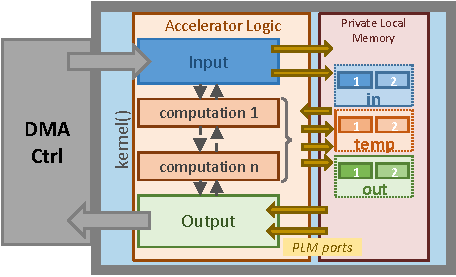
\includegraphics[width=0.5\columnwidth]{fig/accelerator.pdf}
  \caption{Organization of our loosely-coupled accelerators.}\label{fig:accelerator}
\end{figure}

Each accelerator is composed of two parts: the accelerator logic and
the private local memory. The {\bf Accelerator Logic} is composed of
multiple concurrent hardware blocks to manage the data transfers
(e.g. {\em Input} and {\em Output}) and perform the actual computation
(e.g. {\em Computation$_k$}). The {\bf Private Local Memory} (PLM)
locally stores the data structures used by the accelerator to perform
the computation so that they can be accessed with fixed latency by the
accelerator logic. For doing this, it is organized in multiple banks
implemented with area-efficient memory Intellectual Property (IP)
blocks to offer the possibility of multiple concurrent accesses
through different {\em PLM ports}. Each PLM port is connected to a
{\em process interface} in the accelerator logic, which generates the
corresponding memory request.

The rest of this document is organized as follows:
\begin{itemize}
\item Chapter~\ref{ch:methodology} describes the methodology
  implemented by {\sc Mnemosyne};
\item Chapter~\ref{ch:tool} presents the tool, including information
  for installation and configuration;
\item Chapter~\ref{ch:mem_interface} describes the interface of the
  memory IP blocks which is assumed by {\sc Mnemosyne};
\item Chapter~\ref{ch:proc_interface} describes the PLM interface
  generated by {\sc Mnemosyne} to be connected to the rest of the
  accelerator logic.
\end{itemize}



\chapter{Memory Optimization with Mnemosyne}\label{ch:methodology}
To assist the system-level optimization of the memory subsystem for $K$
accelerators, {\sc Mnemosyne} implements the methodology shown in Fig.~\ref{fig:methodology}.
Our methodology takes as input the SystemC descriptions of the accelerators
({\it Accelerator Design$_{1\dots k}$}) and the information about
compatibilities among their data structures ({\it Compatibility Information}).
%

\begin{figure}[h!p]
\centering
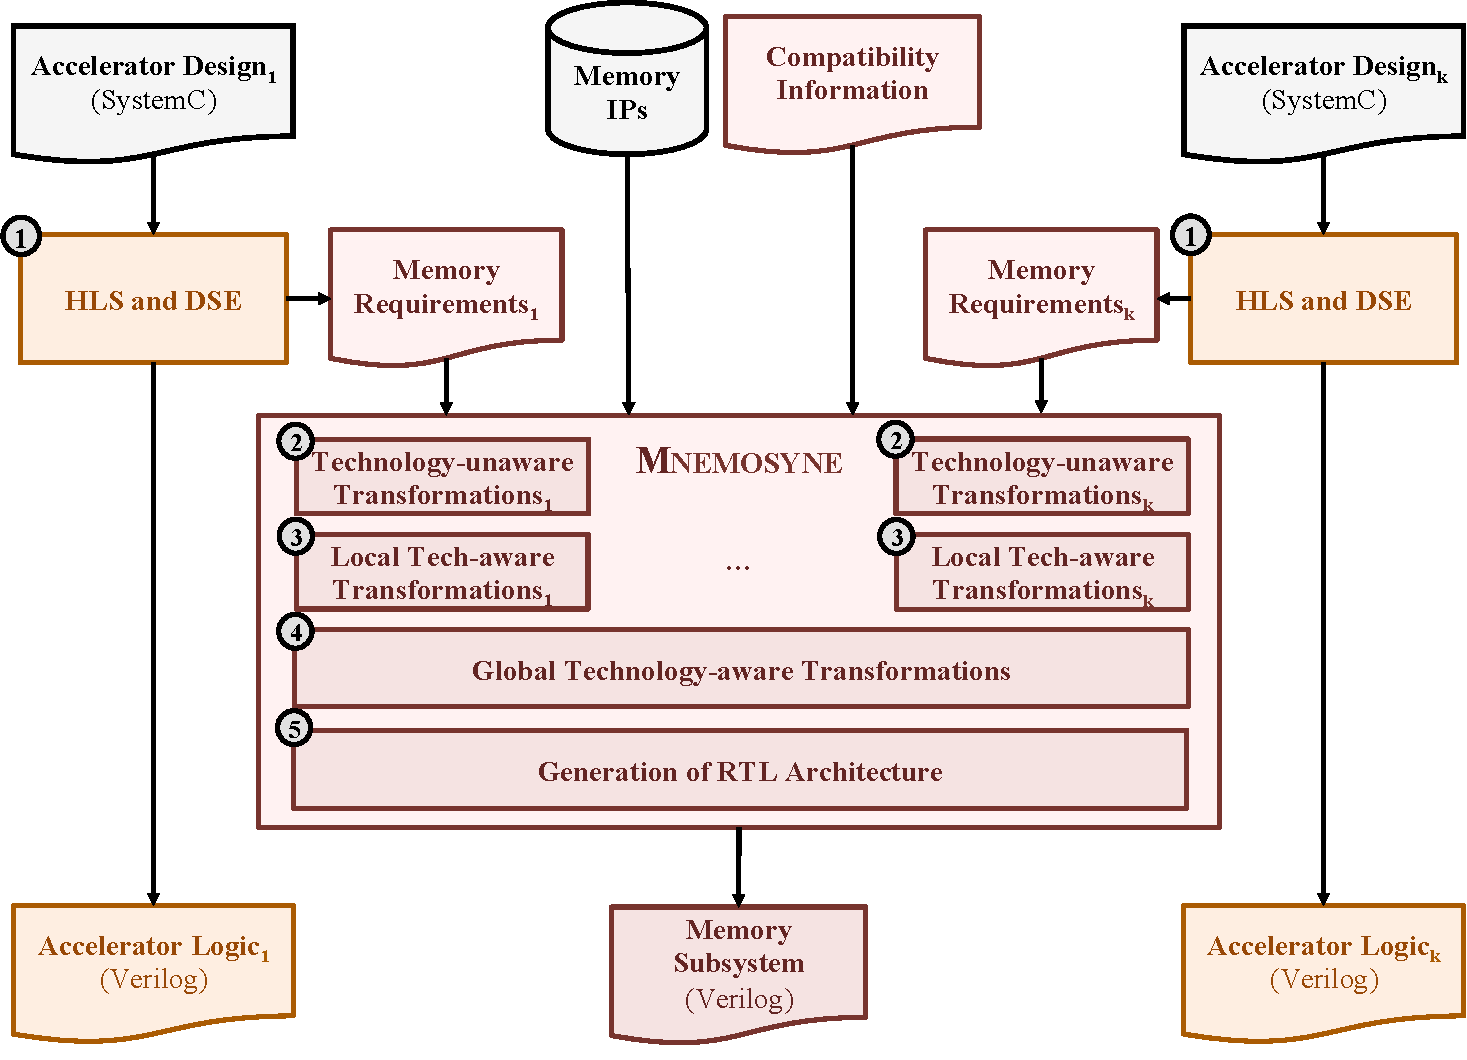
\includegraphics[height=6.4cm]{fig/methodology.pdf}
\caption{Methodology overview for accelerator memory
	design.}\label{fig:methodology}
\end{figure}

We first use a commercial HLS tool to perform design space exploration and generate
many alternative micro-architectures of each accelerator logic in order to
optimize the performance ({\it HLS and DSE}). Each implementation is
characterized by a set of data structures to be stored in the PLM and the
corresponding requirements in terms of memory interfaces ({\it Memory
Requirements$_{1\dots k}$}).
%%
We combine the information on all data structures ({\it Memory Requirements$_{1\dots k}$}),
the information on compatibilities ({\it Compatibility Information}),
and the characteristics of the memory IPs in the
{\it Memory Library} to determine an optimized architecture for each PLM. 
After selecting an implementation for each component, we determine the combined
requirements in terms of memory interfaces to access each data structure in
order to guarantee performance and functional correctness ({\it
Technology-unaware Transformations$_{1\dots k}$}).
%%
First,
we apply transformations for each accelerator ({\it Local Technology-aware
Transformations$_{1\dots k}$}). Then, we consider all accelerators at the same
time and identify when the memory IPs can be reused across different data
structures to minimize the cost of the entire memory subsystem ({\it
Global Technology-aware Transformations}). As output, we produce the RTL
description of the memory subsystem ({\it Generation of RTL Architecture}) that
can be directly integrated with the RTL descriptions of the accelerator logic
generated by the HLS tool.

\section{System-level Memory Optimization}
{\sc Mnemosyne} aims at generating an optimized memory subsystem for
one or more accelerators. The user provides information on the
data structures to be stored in the PLMs, along with additional
information on the number of memory interfaces for each accelerator
and the \textit{compatibilities} between the data structures. This
information is used to share the memory IPs across accelerators
whenever it is possible.
%
Our approach is motivated by the following observations. First, when a data
structure is not used, the associated PLM does not contain any useful data; the
corresponding memory IPs can be reused for storing another data structure, thus
reducing the total size of the memory subsystem.
%%%
Second, in some technologies, the area of a single memory IP is smaller
than the aggregated area of smaller IPs. For example, in an industrial 32nm CMOS
technology, we experimented that a 1,024$\times$32 SRAM is almost 40\%
smaller than the area of two 512$\times$32 SRAMs, due to the replicated logic
for address decoding. In these cases, it is possible to store two data
structures in the same memory IP provided that there are not conflicts on the
memory interfaces, i.e. the data structures are never accessed at the same time
with the same memory operation. Next, we formalize these situations.

To understand when two data structures can share the same memory IPs, we recall
the definition of \textit{data structure lifetime}.
\begin{quote}
{
\small
{\bf Definition.} 
The lifetime of a data structure $b$ is the interval time between the first
memory-write and the last memory-read operations to the data
structure.
\hfill $\blacksquare$
}
\end{quote}
Having two data structures with no overlapping lifetimes means that
while operating on one data structure the other remains unused.
Hence, we can use the same memory IPs to store both of them.  On the other hand,
even when two data structures have overlapping lifetimes, it is still possible
to share memory interfaces to potentially reduce the accelerator area.
\begin{quote}
{
\small
{\bf Definition.} 
Two data structures $b_i$ and $b_j$ are address-space compatible when
their lifetimes are not overlapping for the entire execution of the
accelerator. They are memory-interface compatible when it is possible
to define a \textit{total temporal ordering} of the memory operations so that
two read (resp. write) accesses to $b_i$ and $b_j$ never happen at the
same time.
\hfill $\blacksquare$
}
\end{quote}
When two data structures are memory-interface compatible, memory-read and
memory-write operations are never executed at the same time on the same data
structure.

\section{Data Allocation}

To correctly determine the number and capacity of the memory IPs for a
data structure, we must analyze the data-structure access
patterns and determine how to allocate the data.

If the read patterns can be statically analyzed and are deterministic,
it is possible to distribute the data structure across many
blocks. This technique is called \textit{cyclic partitioning} and
assigns consecutive values of the data structure to different blocks.
%%

Otherwise, it is necessary to create identical copies of the data
({\em data duplication}). This way, each memory-read interface is
assigned to a different block of data and this guarantees to access
the data without conflicts. The corresponding memory-write operations
must create consistent copies of the data in each bank.

\section{Memory Compatibility Graph}

The compatibility information provided by the designer is combined into a
\textit{Memory Compatibility Graph} (MCG), which captures the sharing
opportunities among the data structures.
\begin{quote}
{
\small
{\bf Definition.}
The Memory Compatibility Graph is a graph $MCG=(B,E)$ where each node $b
\in B$ represents a data structure to be stored in the entire memory subsystem;
an edge $e \in E$ connects two nodes when the corresponding data
structures can be assigned to the same physical memory IPs. Each edge $e \in E$
is also annotated with the corresponding type of compatibility (e.g.
address-space or memory-interface).
\hfill $\blacksquare$
}
\end{quote}
%
A MCG with no compatibility edges corresponds to implementing each
data structure in a dedicated PLM element.
%%
Increasing the number of edges into the $MCG$ corresponds to increasing the
number of compatible data structures. This can potentially increase the number
of banks that can be reused across different data structures.
An accurate compatibility graph is the key to optimize the memory subsystem of
the accelerators. In most cases, the designer has to analyze the application's
behavior or modify the interconnection topology of the accelerator to increase
sharing possibilities.


\chapter{Tool Overview}\label{ch:tool}

{\sc Mnemosyne} is a Linux command-line tool that generates the
Verilog code of the PLM controllers based on a set of YAML
configuration files. This chapter describes the tool interface and the
format of these configuration files. It also contains information on
how to configure and install the tool from the source code files.

\section{Tool Interface}

The command-line interface of {\sc Mnemosyne} is the following:

\begin{verbatim}
              .:: Mnemosyne ::.
 Columbia University, Copyright (c) 2014-2017

Revision: 55fc8cf7a9d90f6610fffa7d61e1c2dff4b4c596(master)

 == Command-line parameters:

General options:
  --help                                Print help message
  -v [ --verbosity ] arg (=0)           Verbosity level
  --config arg                          Configuration file

Input options:
  --name arg                            Name of the component
  --memlib arg                          Library of memory IPs (YAML)
  --mode arg (=opt)                     Execution mode (batch, opt)
  --opt-goal arg (=AREA_HEURISTIC)      Optimization goal:
                                          AREA_HEURISTIC: Area Minimization
  --disable-optimization arg            Disable specific optimizations
                                        (COLORING,ADDRESS_SPACE,INTERFACE)

Batch-mode options:
  --interfaces arg                      List of memory interfaces
  --width arg                           Array bitwidth
  --height arg                          Array height (in words)

Optimization-mode options:
  --input-cgraph arg                    Compatibility graph (YAML)
  --acc-config arg                      Accelerator configuration (YAML)
  --acc-interface arg                   Accelerator interface (YAML)
  --acc-list arg                        List of accelerators' configurations
                                        (YAML)

Output options:
  --target-verilog-dir arg (=./output)  Output directory (Verilog files)
  --verilog-name arg                    Verilog filename (memory subsystem)
  --temp-dir arg (=./work)              Temporary directory
  --export arg                          Export mode:
                                          IPXACT: Vivado IP-XACT component
                                          CTOSIP: Cadence C-to-Silicon vendor
                                                  RAM
                                          STRATUSIP: Cadence Stratus memory IP
  --generate-top-plm arg (=0)           Generate top module of memory subsystem
  --top-name arg                        Name of top module
  --top-verilog-name arg                Verilog filename (top module)
  --target-export-dir arg (=./output)   Output directory (Export files)
\end{verbatim}

\noindent Specifically, the general options are:
\begin{itemize}
\item {\tt help} prints the above message window.
\item {\tt verbosity} indicates the verbosity level for the tool. The
  default level only reports minimal information, like the number of
  generated PLM controllers and the total area of the resulting memory
  subsystem.  Increasing the verbosity level allows the user to get
  additional information about the tool execution.
\item {\tt config} specifies the YAML configuration file, whose options can
  be then overwritten with explicit command-line options (see Section~\ref{sec:config}).
\end{itemize}

\noindent The input options for all execution modes are:
\begin{itemize}
\item {\tt name} specifies the name of the accelerator. It is used to
  eventually determine the name of the top component and the file containing the generated
  memory subsystem.
\item {\tt memlib} specifies the YAML file of the memory library (i.e. list of
  available memory IP blocks) to be used for creating the accelerator memory
  subsystem (see Section~\ref{sec:library}).
\item {\tt mode} specifies the execution mode:
\begin{itemize}
\item {\tt batch}: only one single memory IP is generated;
\item {\tt opt}: multiple data structures are analyzed for identifying sharing opportunities.
\end{itemize}
\item {\tt opt-goal} specifies which is the algorithm used to perform optimization:
\begin{itemize}
\item AREA\_HEURISTIC: area minimization (default)
\end{itemize}
\item {\tt disable-optimization} specifies that the given optimization must be disabled. This option can be repeated several times with different values:
\begin{itemize}
\item COLORING: disabling the interface coloring optimization;
\item ADDRESS\_SPACE: disabling the sharing of data structures with compatibile address spaces;
\item INTERFACE: disabling the sharing of data structures with compatibile interfaces.
\end{itemize}
\end{itemize}

\noindent The options for the batch-mode execution are:
\begin{itemize}
\item {\tt interfaces} specifies the list of interfaces for the memory block to be generate.
\item {\tt width} specifies the width (in bits) of the data to be stored.
\item {\tt height} specifies the number of data words to be stored.
\end{itemize}

\noindent The options for the optimization-mode execution are:
\begin{itemize}
\item {\tt input-cgraph} specifies the YAML file describing the compatibilities among the data structures to be stored into the PLM (see Section~\ref{sec:compatibility}).
\item {\tt acc-config} specifies the YAML file containing the data
  structures to be stored into the PLM (see Section~\ref{sec:config}).
\item {\tt acc-interface} specifies the YAML file containing the
  interface of the component to be
  attached to the generated memory subsystem (see
  Section~\ref{sec:interface}).
\item {\tt acc-list} specifies the YAML file containing the
  configurations of the accelerators to be optimized concurrently (see
  Section~\ref{sec:multi-acc}).
\end{itemize}

\noindent The output options for all execution modes are:
\begin{itemize}
\item {\tt target-verilog-dir} specifies which is the directory where the
  output files will be generated.
\item {\tt verilog-name} specifies the name of the output Verilog file that will be generated.
\item {\tt temp-dir} specifies the name of the temporary directory.
\item {\tt export} specifies the export modes to be activated. This option can be repeated several times with different values:
\begin{itemize}
\item IPXACT: description of the memory IP in IP-XACT format suitable for Xilinx Vivado Design Suite;
\item CTOSIP: description of the memory IP in the vendor RAM format suitable for Cadence C-to-Silicon;
\item STRATUSIP: description of the memory IP in the vendor RAM format suitable for Cadence Stratus HLS.
\end{itemize}
\item {\tt generate-top-plm} specifies whether the top PLM module (i.e., the one containing all the PLM modules) has to be generated.
\item {\tt top-name} specifies the name of the top module containing the PLM modules and the component to be connected.
\item {\tt top-verilog-name} specifies the name of the Verilog file containing the top module to be generated.
\item {\tt target-export-dir} specifies which is the directory where the
 files generated by the export mode will be generated.
\end{itemize}
  
\section{Configuration, Installation, and Execution}

{\sc Mnemosyne} has been implemented in C++\footnote{The current
  source files can be found at:
  \mygit{https://github.com/chrpilat/mnemosyne} (branch
        {\em master})} and tested under Linux 16.04 LTS.
{\sc Mnemosyne} requires the following libraries for compilation and
execution:
\begin{itemize}
\item python-networkx
\item libboost-all-dev
\item libxml++2.6-dev
\item glpk-utils
\end{itemize}
The tool can be configured and installed using CMake. One nice and
highly recommended feature of CMake is the ability to do out-of-source
builds. In this way you can make all your object files, various
temporary depend files, and even the binary executables without
cluttering up your source tree. To use out-of-source builds, create a
build directory in your top-level folder (technically, this can be
anywhere, but the top-level project folder seems to be a logical
choice). Next, change into your build directory and run {\tt cmake}
pointing it to the directory of the top-level CMakeLists.txt.  For
example, the following set of commands configures {\sc Mnemosyne} so
that the executable will be installed in {\sc /opt/mnemosyne/bin}, while
the YAML files of the available memory libraries will be installed in
{\sc /opt/mnemosyne/share}:

\begin{commandshell}{Path: <mnemosyne\_top>}
  mkdir build
  cd build
  cmake .. -DCMAKE_INSTALL_PREFIX=/opt/mnemosyne
\end{commandshell}

\noindent The tool can be then compiled and installed with the
following commands:

\begin{commandshell}{Path: <mnemosyne\_top>/build}
  make
  make install
\end{commandshell}

\noindent After installation, the current version of the memory
libraries will be available in the directories {\tt
<target\_path>/share/tech/<tech>} (for each target technology {\tt
tech}). These directories will contain the Verilog files of the wrappers
around the memory IPs (see Chapter~\ref{ch:mem_interface}) and the YAML file
containing the list of available memory IPs, along with technology-related
information (e.g. area).

\subsection{Execution Modes}

The tool has several execution modes, where the designer must specify the
name of the accelerator and the YAML file of
the corresponding memory library. Additional parameters for each execution mode
are detailed below.

\vspace{4pt}
{\bf Batch execution.} This mode generates a memory IP for a single data structure. For example,
if the designer wants to generate a PLM for a 1,024$\times$32 array (one write and one read interfaces), the tool can be invoked as 
follows (see the example in the folder \name{examples/batch}):

\begin{commandshell}{}
  mnemosyne --mode batch --memlib /opt/mnemosyne/share/tech/virtex7/virtex7_memlib.yaml  \                 --width 32 --height 1024 --interfaces w,r --name plm_1024x32_1w1r
\end{commandshell}

\noindent This command generates the Verilog file {\tt mem\_plm\_1024x32\_1w1r\_rtl.v} of the corresponding memory subsystem. This file is generated in the subfolder {\tt output} (i.e. the default one).

\vspace{4pt}
{\bf Single-accelerator optimization.} This mode requires to specify
the accelerator configuration and the compatibility graph. For
example, if the designer wants to generate a PLM for the
accelerator {\sc Sort} targeting an FPGA technology, the tool can be
invoked as follows (see the example in the folder \name{examples/multiacc}):

\begin{commandshell}{}
  mnemosyne --memlib /opt/mnemosyne/share/tech/virtex7/virtex7_memlib.yaml  \                 --acc-config ./sort_0_config.yaml --input-cgraph ./sort_cgraph.yaml --name sort
\end{commandshell}

\noindent This command generates the Verilog file {\tt mem\_sort\_rtl.v} of the corresponding memory subsystem. This file is generated in the subfolder {\tt output} (i.e. the default one).

\vspace{4pt}
{\bf Single-accelerator optimization with top module generation.} In order to
generate the top module that connects the memory subsystem and the accelerator
logic, it is necessary to specify the YAML file containing the description of the
module interface. For example, to generate both the PLM and the
corresponding top module for the {\sc Sort} accelerator, {\sc Mnemosyne} can be
invoked as follows (see the example in the folder \name{examples/multiacc}):

\begin{commandshell}{}
  mnemosyne --memlib /opt/mnemosyne/share/tech/virtex7/virtex7_memlib.yaml  \                 --acc-config ./sort_0_cfg.yaml --input-cgraph ./sort_cgraph.yaml --name sort \
        --acc-interface ./sort_0_interface.yaml \end{commandshell}

\noindent This command generates two Verilog files ({\tt mem\_sort\_rtl.v}
and {\tt top\_sort\_rtl.v}, respectively). The former contains the
generated memory subsystem, while the latter contains the interconnections
between the accelerator logic and the different PLM controllers that have been
generated.  The files are generated in the subfolder {\tt output} (i.e. the
default one).

\vspace{4pt}
{\bf Multi-accelerator optimization.} In order to share the memory IPs across
multiple accelerators, it is necessary to specify the list of accelerators and
the corresponding configuration files. This configuration specifies also the
order of the accelerators, whose identifier is used in the device driver to
configure and start the execution of the corresponding accelerator. For creating the
memory subsystem and the top module of two accelerators {\sc Sort} and {\sc
Debayer}, {\sc Mnemosyne} can be invoked as follows (see the example in the folder \name{examples/multiacc}):

\begin{commandshell}{}
  mnemosyne --memlib /opt/mnemosyne/share/tech/virtex7/virtex7_memlib.yaml  \                 --acc-list ./multiacc_config.yaml --name multiacc
\end{commandshell}

\begin{lattention}
{\sc Mnemosyne} assumes that the accelerators are never executed at the same
time and it is not necessary to preserve data between the execution of the
accelerators. Hence, each data structure of an accelerator is compatible with 
the data structures of any other accelerator.
\end{lattention}

\noindent This command generates a Verilog file containing the unique memory
subsystem for all accelerators ({\tt mem\_multiacc\_rtl.v}) and a
Verilog file for the top module with the logic to drive all the accesses to the
DMA controller and the configuration registers ({\tt
top\_multiacc\_rtl.v}).

\section{Memory Library}\label{sec:library}

The memory library contains the list of memory IPs that are available to create
the multi-bank architecture of the accelerator memory subsystem and store all
the data structures.  Besides default memory libraries, it is possible to
defined user-specific libraries with a custom set of memory IPs, including more
complex macro-blocks.

This section describes how to specify a memory library to be used by {\sc
Mnemosyne} when creating the accelerator memory subsystem. A custom library can
be specified in YAML as follows:

\begin{myxml}{File: ./memory\_library.yaml}
name: mymemorylibrary
memory_ip:
 - type           : [...]
   [...]
 - type           : [...]
   [...]
 - type           : [...]
   [...]
 - type           : [...]
   [...]
\end{myxml}
\noindent This memory library contains four memory IPs, each of them represented by the tag {\tt type} with 
the name of the memory IP.
Indeed, each tag {\tt memory\_ip} represents a memory IP block that can be used by
the tool. This tag must have the following elements:
\begin{itemize}
\item {\tt width} represents the bitwidth of the data to be stored;
\item {\tt height} represents the number of elements that can be stored in the memory IP;
\item {\tt file} indicates the Verilog file that contains the defintion of the component that wraps the
actual memory IP provided by the technology vendor (see
Chapter~\ref{ch:mem_interface});
\item {\tt area} indicates the resource requirements for this memory IP (e.g. $um^2$ in case
of CMOS technology or number of BRAMs in case of FPGA technology);
\item {\tt interfaces} specifies the list of interfaces offered by the memory IP. Each of them can be specified as``r'' (read-only), ``w'' (write-only), or ``rw'' (read/write).
\end{itemize}
For example, a dual-port memory IP for CMOS technology capable to store 1,024 32-bit elements can be specified 
as follows:
\begin{myxml}{File: ./memory\_library.yaml}
 - type           : SRAM_1024x32
   height         : 1024
   width          : 32
   interfaces     : [rw, rw]
   area           : [...]
   file           : [...]
\end{myxml}
\noindent A PLM controller that is implemented with this memory IP will contain a certain
number of modules named {\tt SRAM\_1024x32}, whose definition is specified
inside the given file.

\section{Accelerator Configuration}\label{sec:config}

This section describes the format of the YAML file that is used to specify which
data structures have to be stored in the PLM, along with the associated
information necessary to create the proper micro-architecture of the memory
subsystem. The file is organized as follows:
\begin{myxml}{File: <accelerator>.yaml}
arrays:
  - name       : [...]
    [...]
  - name       : [...]
    [...]
  - name       : [...]
    [...]
\end{myxml}
\noindent where each tag {\tt name} represents a data structure to be stored in the PLM.
Each of these tags must have the following attributes:
\begin{itemize}
\item {\tt name} represents the name of the data structure;
\item {\tt width} represents the bitwidth of the data structure;
\item {\tt height} represents the number of elements to be stored;
\item {\tt interfaces} specifies the list of all interfaces required by the processes of the accelerator logic to access the data structure. 
\end{itemize}

\begin{lattention}
{\sc Mnemosyne} assumes a specific order of the interfaces: write interfaces must be specified
first, followed by read/write interfaces, and then read interfaces.
\end{lattention}

\vspace{4pt}
{\bf Buffer definition.}
Each buffer must also contain information about the processes that
access the data structure, along with details about the corresponding interfaces
and the access pattern. The list of processes is specified as follows:

\begin{myxml}{File: <accelerator>.yaml}
  - name       : [...]
    [...]
    processes  :
      - name       : [...]
        [...]
\end{myxml}
\noindent where each tag {\tt process} has the following attributes:
\begin{itemize}
\item {\tt name} represents the name of the process 
\item {\tt interfaces} specifies which interfaces (positional index with respect to the general list) are used by the current process;
\item {\tt read\_pattern} specifies the access pattern for the read interfaces of the current process (optional);
\item {\tt write\_pattern} specifies the access pattern for the write interfaces of the current process (optional).
\end{itemize}
For example, let us assume to have a 2,048 16-bit array named {\tt
A0}, which is written by process {\tt producer} with one interface and
read by process {\tt consumer} with two interfaces. The buffer is then
specified as follows:
\begin{myxml}{File: <accelerator>.yaml}
  - name       : A0
    height     : 2048
    width      : 16
    interfaces : [w, r, r]
    processes  :
      - name       : producer
        interfaces : 0
      - name       : consumer
        interfaces : [1, 2]
\end{myxml}

\vspace{4pt}
{\bf Interface sharing.}
Additional tags can be used to specify compatibility between the interfaces. For
example, let {\tt B0} be a data structure written by process {\tt producer} and
read by two processes {\tt consumer\_one} and {\tt consumer\_two} executing
serially. The buffer is then defined as follows:
\begin{myxml}{File: <accelerator>.yaml}
  - name       : B0
    height     : 2048
    width      : 16
    interfaces : [w, r, r]
    processes  :
      - name       : producer
        interfaces : 0
      - name       : consumer_one
        interfaces : 1
      - name       : consumer_two
        interfaces : 2
\end{myxml}
\noindent Then, since the two read processes never access the data structure at the same time,
it is possible to specify that interfaces {\tt 1} and {\tt 2} can be shared. This can 
be specified by adding the tag {\tt sharing} as follows:
\begin{myxml}{File: <accelerator>.yaml}
  - name       : B0
    height     : 2048
    width      : 16
    interfaces : [w, r, r]
    processes  :
      - name       : producer
        interfaces : 0
      - name       : consumer_one
        interfaces : 1
      - name       : consumer_two
        interfaces : 2
    sharing    : [1, 2]
\end{myxml}
\noindent{\sc Mnemosyne} then generates a PLM micro-architecture that minimizes the
memory IPs with the proper logic to drive the requests from the processes.

\section{Memory Compatibility Graph}\label{sec:compatibility}

The memory compatibility graph specifies the relationships among the data
structures. The graph is represented by a text file that is organized as
follows:
\begin{myxml}{File: <accelerator>.yaml}
nodes: [...]
edges:
  - compatibility : [...]
    type          : [...]
  - compatibility : [...]
    type          : [...]
  - compatibility : [...]
    type          : [...]
\end{myxml}
\noindent where the tag {\tt nodes} represents the list of nodes to be
stored in the PLM, while the tag {\tt edges} denotes the list of compatibility edges (i.e., each pair of two compatible nodes).

\begin{lattention}
The list of nodes in the memory compatibility graph must match the
list of data structures in the configuration
file. Specifically, the memory compatibility graph must contain one
node for each of the data structures.
\end{lattention}

\noindent The list of nodes is specified as follows:
\begin{myxml}{File: <accelerator>.yaml}
nodes : [A0, A1, A2]
\end{myxml}
\noindent where the names of the data structures are reported in the list. Note that there has to be at least a tag with name {\tt A0} in the configuration file of the
accelerator.
An edge is specified instead as follows:
\begin{myxml}{File: <accelerator>.yaml}
edges:
    [...]
    - compatibility : [A0, A1]
      type          : b
    [...]
\end{myxml}
\noindent where the tag {\tt compatibility} contains the pair of nodes, while the text contained in 
the tag {\tt type} specifies the type of
compatibility. Currently, the following types are supported: {\em address-space
compatibility} (type {\bf a}) and {\em memory-interface compatibility} (type
{\bf b}).
\begin{lattention}
{\sc Mnemosyne} adopts a conservative approach. Hence, if there is no
edge between two nodes, the tool assumes that the two corresponding
data structures are not compatible and behaves accordingly (e.g. it
does not share memory IPs between the two nodes).
\end{lattention}

\section{Accelerator Interface}\label{sec:interface}

The YAML file describing the accelerator interface is used to generate the
connection between process interfaces (defined in
Chapter~\ref{ch:proc_interface}) and the corresponding interfaces of
the generated PLM controllers. This is simply a translation of the
Verilog/VHDL interface of the module.
%%%
The file is organized as follows:
\begin{myxml}{File: <accelerator>\_rtl.yaml}
name: [...]
interface:
   - id: [...]
     [...]
   - id: [...]
     [...]
\end{myxml}
\noindent where each tag {\tt id} specifies the name of a port of the module (as indicated in the
corresponding Verilog/VHDL file). Each tag must have the following attributes:
\begin{itemize}
\item {\tt dir} specifies the direction of the port (either ``input'' or ``output'');
\item {\tt size} specifies the size of the port (in bits).
\end{itemize}

Examples of port descriptions are shown below:
\begin{myxml}{File: <accelerator>\_rtl.yaml}
name: [...]
interface:
   - id  : clk
     dir : input
     size: 1 
   [...]
   - id  : A0_D0
     dir : output
     size: 32 
   [...]
   - id  : A1_Q0
     dir : input
     size: 32
\end{myxml}
\noindent where the clock port is defined as a single-bit input port, while the data ports of two memory interfaces for accessing a 32-bit data structures have the corresponding direction and size.

\section{Multi-accelerator Optimization}\label{sec:multi-acc}

{\sc Mnemosyne} can be also used to optimize the memory subsystem of multiple
accelerators executing in time multiplexing. For this, it is necessary to
specify a YAML configuration file, which contains information (i.e. accelerator
configuration, interface, and compatibility graph) about each accelerator.
%%%
The file has the following format:
\begin{myxml}{File: <accelerators>.yaml}
accelerator:
  - name          : [...]
    [...]
  - name          : [...
    [...]
\end{myxml}
\noindent where each tag {\tt name} contains the name and the description of an
accelerator that shares the memory IPs with all the others. Note that the
positional index of the accelerators in this list corresponds to the id used for
the configuration of the macro-block by the device driver.
%%
Each of these tags must have the following attributes:
\begin{itemize}
\item {\tt cgraph} is the path to the compatibility graph of the accelerator
(see Section~\ref{sec:compatibility});
\item {\tt acc\_config} represents the path to the accelerator configuration
(see Section~\ref{sec:config});
\item {\tt acc\_interface} contains the path to the accelerator interface (see
Section~\ref{sec:interface}).
\end{itemize}
\noindent In this execution mode, {\sc Mnemosyne} does not require any changes to the configuration files of each single accelerator. So the suggested approach is:
\begin{enumerate}
\item generate the configuration files for each single accelerator;
\item validate the generated memory subsystem with RTL simulation;
\item create the configuration file for multi-accelerator optimization by wrapping 
these generated configuration files for each single accelerator.
\end{enumerate}
\noindent Let {\sc Sort} and {\sc Debayer} be two accelerators to be executed in
time multiplexing as in the example contained in the folder \name{example/multiacc}. We can create a single macro-accelerator called {\sc multiacc}
with a unique memory subsystem by executing {\sc Mnemosyne} as follows:
\begin{commandshell}{}
  mnemosyne --memlib /opt/mnemosyne/share/tech/virtex7/virtex7_memlib.yaml  \                 --acc-list ./multiacc_config.yaml --name multiacc
\end{commandshell}
\noindent where the file {\tt multiacc\_config.yaml} is organized as follows:
\begin{myxml}{File: example/multiacc\_config.yaml}
accelerator:
  - name          : sort_0
    cgraph        : ./sort_cgraph.yaml
    acc_config    : ./sort_0_config.yaml
    acc_interface : ./sort_0_interface.yaml
  - name          : debayer_0
    cgraph        : ./debayer_cgraph.yaml
    acc_config    : ./debayer_0_config.yaml
    acc_interface : ./debayer_0_interface.yaml
\end{myxml}

\section{Configuration File}\label{sec:config}

{\sc Mnemosyne} also supports configuration files with a subset of the parameters. This is particularly useful when Mnemosyne has to be executed multiple times with different values only for part of the parameters. For example, {\sc Mnemosyne} can be used to design several 1,024$\times$32 memories with the following configuration file:

\begin{myxml}{File: config.cfg}
mode               = batch
memlib             = /opt/mnemosyne/share/tech/virtex7/virtex7_memlib.yaml
height             = 1024
width              = 32
\end{myxml}
\noindent where each command-line parameter is stored in the form \name{<parameter_name> = <parameter_value>}. Then, {\sc Mnemosyne} can be invoked as follows:

\begin{commandshell}{}
  mnemosyne --config config.cfg --interfaces w,r --name mem_1024x32_1w1r
  mnemosyne --config config.cfg --interfaces w,r,r --name mem_1024x32_1w2r
  mnemosyne --config config.cfg --interfaces w,r,r,r,r --name mem_1024x32_1w4r
\end{commandshell}

The parameters in the configuration file can be overwritten by redefining the value in the command line. For example, an alternative 512$\times$32 memory can be designed as follows:
\begin{commandshell}{}
  mnemosyne --config config.cfg --interfaces w,r --height 512 --name mem_512x32_1w1r
\end{commandshell}




\chapter{Memory Block Interface}\label{ch:mem_interface}
This chapter describes the interface that {\sc Mnemosyne} assumes for
each memory IP. This can be used to create the wrappers for new
technologies or to extend the memory library with IPs that are
composed of multiple blocks.
%%
Given a memory IP with parameters {\tt width} and {\tt height}, {\sc
  Mnemosyne} assumes that its interface features the following global
signal:
\begin{itemize}
\item {\tt CLK} represents the clock signal for all interfaces.
\end{itemize}
\noindent Currently, there are no explicit signals to reset the memory IP. Hence, 
the designer must ensure that data are never read before being written.
\begin{lattention}
  Currently, {\sc Mnemosyne} does not support memory interfaces with
  independent clocks. Hence, if the memory IP has separated clocks for
  each interface, they must be connected to the same input signal.
\end{lattention}

\noindent Then, let $n$ be the index of the memory interface, {\sc
  Mnemosyne} assumes that the memory interface $n$ has the following
signals:
\begin{itemize}
\item {\tt An} (input) represents the physical address to be accessed
  inside the memory IP. This signal has a size of {\tt
    $log_2(height)$} bits;
\item {\tt CEn} (input, active high) indicates that an operation
  (either read or write) is active on the current memory IP. This
  signal has a size of one bit.
\item {\tt WEn} (input, active high) indicates that the memory IP is
  accessed for a write operation. This signal has a size of one bit.
\item {\tt Dn} (input) specifies the input data to be written (for
  write operations). This signal has a size of $width$ bits.
\item {\tt WEMn} (input) indicates the mask for write operations
  (i.e. which bits of the input data have to be effectively
  written). This signal has a size of $width$ bits.
\item {\tt Qn} (output) is the output value produced by a read
  operation. This signal has a size of $width$ bits.
\end{itemize}

\begin{lattention}
  The write mask feature (signal {\tt WEMn}) is not available in all
  technologies. For example, in FPGA, all bits of the input data are
  always written, regardless of the value of this signal, which is
  ignored.
\end{lattention}

\noindent Note that signals {\tt WEn}, {\tt WEMn}, and {\tt Dn} are
available only for write interfaces, while signal {\tt Qn} is
available only for read interfaces. All signals are available,
instead, for read/write interfaces.

\newpage

For example, a dual-port 1024$\times$32 memory IP for CMOS technology,
named {\tt SRAM\_1024x32}, has the following module interface:

\begin{myverilog}{}
module SRAM_1024x32 (CLK, CE0, A0, WE0, D0, WEM0, Q0, CE1, A1, WE1, D1, WEM1, Q1 );
  input         CLK;
  //first interface
  input         CE0;
  input  [9:0]  A0;
  input         WE0;
  input  [31:0] D0;
  input  [31:0] WEM0;
  output [31:0] Q0;
  //second interface
  input         CE1;
  input  [9:0]  A1;
  input         WE1;
  input  [31:0] D1;
  input  [31:0] WEM1;
  output [31:0] Q1;
  //definition of the macro given by the technology vendor
  //...
endmodule 
\end{myverilog}

\noindent Hence, it is possible to use the so-created wrappers to create complex
memory blocks by instantiating multiple replica of these modules and creating
the proper logic to drive each of the signals. For example, let {\tt A0} be a
2048$\times$32 array to be stored in the PLM with one memory-ready and one
memory-write interface. The correponding memory block is defined as follows:

\begin{myverilog}{}
module array_A0 (CLK, CE0, A0, WE0, D0, WEM0, Q0, CE1, A1, Q1 );
  input         CLK;
  //first interface
  input         CE0;
  input  [10:0] A0;
  input         WE0;
  input  [31:0] D0;
  input  [31:0] WEM0;
  //second interface
  input         CE1;
  input  [10:0] A1;
  output [31:0] Q1;
  //logic to drive interface signals from/to IP ports
  //...
  //definitions of the banks
  SRAM_1024x32 mem_0(.CLK(CLK), .CE0(mem_0_CE0), .A0(mem_0_A0),
      .D0(mem_0_D0), .WE0(mem_0_WE0), .WEM0(mem_0_WEM0), .Q0(mem_0_Q0),
      .CE1(mem_0_CE1), .A1(mem_0_A1), .Q1(mem_0_Q1),
      .D1(mem_0_D1), .WE1(mem_0_WE1), .WEM1(mem_0_WEM1));     
  SRAM_1024x32 mem_1(.CLK(CLK), .CE0(mem_1_CE0), .A0(mem_1_A0),
      .D0(mem_1_D0), .WE0(mem_1_WE0), .WEM0(mem_1_WEM0), .Q0(mem_1_Q0),
      .CE1(mem_1_CE1), .A1(mem_1_A1), .Q1(mem_1_Q1),
      .D1(mem_1_D1), .WE1(mem_1_WE1), .WEM1(mem_1_WEM1));
endmodule 
\end{myverilog}

\noindent Where the different signals \name{mem_0_XX} and \name{mem_1_XX} represent the
logic necessary to drive the ports of the two memory IPs, respectively. This
logic is then automatically generated by {\sc Mnemosyne} based on the memory
requirements. For example, since we must apply {\em block partitioning} to
allocate the array to these memory blocks, a memory-read operation is activated
on the second interface of the memory IP \name{mem_0} when the most significant
bit is zero. Similarly, the memory-read operation is activated on the memory
IP \name{mem_1} when the most significant bit is one. The rest of the address is
used to specify the offset to access the data inside the memory IP.

\begin{myverilog}{}
  assign mem_0_CE1 = (C1 & A1[10:10] == 0) ? 1'b1 : 1'b0;
  assign mem_0_A1 = (C1 & A1[10:10] == 0) ? A1[9:0] : {10{1'b0}};
  assign mem_1_CE1 = (C1 & A1[10:10] == 1) ? 1'b1 : 1'b0;
  assign mem_1_A1 = (C1 & A1[10:10] == 1) ? A1[9:0] : {10{1'b0}};
\end{myverilog}






\chapter{PLM Controller Interface}\label{ch:proc_interface}
This chapter describes the interface that {\sc Mnemosyne} assumes for
the process interfaces of the accelerator logic. This can be used to
create components that can interface with the generated memory
wrappers.
%%
Given a process interface $n$ used to access a data structure of parameters {\tt width} and {\tt height}, {\sc
  Mnemosyne} assumes that the interface features the following signals:
\begin{itemize}
\item {\tt An} (output) represents the offset inside the data structure
(i.e. the logical address) to be accessed with the memory operation.  This
signal has a size of {\tt $log_2(height)$} bits;
\item {\tt CEn} (output, active high) indicates that there is an active
request on the current process interface (i.e. a memory operation is accessing
the corresponding data structure). This signal has a size of one bit.
\item {\tt WEn} (output, active high) indicates that there is an active
memory-write operation on the interface.  The input data is assumed to be valid
in this case. This signal has a size of one bit.
\item {\tt Dn} (output) specifies the data to be written (for
  write operations). This signal has a size of $width$ bits.
\item {\tt WEMn} (output) indicates the mask for write operations
  (i.e. which bits of the input data have to be effectively written). This
  signal has a size of $width$ bits.
\item {\tt Qn} (input) is the output value produced by a read
  operation. This signal has a size of $width$ bits.
\end{itemize}

\noindent Note that signals {\tt WEn}, {\tt WEMn}, and {\tt Dn} are
available only for write interfaces, while signal {\tt Qn} is
available only for read interfaces. All signals are available,
instead, for read/write interfaces.

{\sc Mnemosyne} generates the logic to translate the memory requests into
proper memory requests to the physical memory IPs necessary to store the
corresponding data structure. Specifically, it generates a PLM controller that
contains a configuration of memory IPs that can store the corresponding data
structure (more than one in case of bank reuse). This PLM controller has as many
interfaces as the ones requested by the accelerator logic. It contains
internally the logic for address translation.

For example, a component \name{accelerator_logic} that needs to access
a 2048$\times$32 array named {\tt A0} with two memory interfaces (one
write and one read interface) has the interface:

\begin{myverilog}{}
module accelerator_logic (CLK,
              //...
              A0_CE0, A0_A0, A0_WE0, A0_D0, A0_WEM0,
              A0_CE1, A0_A1, A0_Q1,
              //...
              );
  input         CLK;
  //.. other signals / interfaces
  //write interface
  output        A0_CE0;
  output [10:0] A0_A0;
  output        A0_WE0;
  output [31:0] A0_D0;
  output [31:0] A0_WEM0;
  //read interface
  output        A0_CE1;
  output [10:0] A0_A1;
  input  [31:0] A0_Q1;
  //... other signals / interfaces
  //... rest of the module
endmodule 
\end{myverilog}


\noindent This module can be simply connected to the corresponding PLM 
(see Section~\ref{ch:mem_interface} for its definition) with direct
signals as follows:

\begin{myverilog}{}
module accelerator (CLK,
              //...
              //other signal / interfaces
              //...
              );
  input         CLK;
  //.. other signals / interfaces
  //write interface signals
  wire        A0_CE0;
  wire [10:0] A0_A0;
  wire        A0_WE0;
  wire [31:0] A0_D0;
  wire [31:0] A0_WEM0;
  //read interface
  wire        A0_CE1;
  wire [10:0] A0_A1;
  wire [31:0] A0_Q1;
  //accelerator logic
  accelerator_logic acc_0(.CLK(CLK), 
      //...other signals / interfaces 
      .A0_CE0(A0_CE0), .A0(A0_A0),
      .A0_D0(A0_D0), .A0_WE0(A0_WE0), .A0_WEM0(A0_WEM0), 
      .A0_CE1(A0_CE1), .A0_A1(A0_A1), .A0_Q1(A0_Q1));     
  //PLM
  array_A0 mem_0(.CLK(CLK),
      .CE0(A0_CE0), A0(A0_A0), 
      .D0(A0_D0), .WE0(A0_WE0), .WEM0(A0_WEM0),
      .CE1(A0_CE1), A1(A0_A1), .Q1(A0_Q1));
endmodule 
\end{myverilog}


\end{document}
